\documentclass[aspectratio=169]{beamer}
\usetheme{Madrid}
\usecolortheme{seahorse}
\setbeamertemplate{navigation symbols}{}
\setbeamertemplate{footline}[frame number]
\setbeamersize{text margin left=8mm,text margin right=8mm}

\usepackage{amsmath,amssymb,bm}
\usepackage{braket}
\usepackage{booktabs}
\usepackage{graphicx}
\usepackage{tikz}
\usetikzlibrary{arrows.meta,positioning,calc}
\setlength{\abovedisplayskip}{5pt}
\setlength{\belowdisplayskip}{5pt}

\title{Generative quantum advantage for classical and quantum problems}
\author{}
\institute{Quantum Machine Learning}
\date{\today}

\begin{document}

\begin{frame}
  \maketitle
\end{frame}

% \begin{frame}{Outline}
%   \begin{itemize}
%     \item Background \& Claim
%     \item This Work
%     \item Task 1: Learning Classically Intractable Distributions
%     \item Task 1: Experiments \& Results
%     \item Task 2: Learning Quantum Circuits for Accelerated Physical Simulation
%     \item Takeaway
%   \end{itemize}
% \end{frame}

\section{Background \& Claim}

\begin{frame}{Beyond-Classical Sampling: Status and Gap}
  \begin{block}{Established fact}
    Beyond-classical quantum experiments have shown that quantum devices can sample from distributions that are classically intractable to simulate.
  \end{block}
\vspace{0.3em}
  \begin{alertblock}{Critical gap}
    Complexity barriers have thwarted efficient learning of such distributions.
  \end{alertblock}

  % \vspace{0.3em}
  % \begin{itemize}
  %   \item Demonstrating hard sampling alone is not sufficient.
  %   \item We must also show the target distribution can be learned and generated reliably.
  % \end{itemize}
\end{frame}

\begin{frame}{A Stronger Definition of Generative Quantum Advantage}
  \begin{block}{Goal emphasized in this talk}
    {\bfseries Generative quantum advantage}: quantum computers can \textbf{learn and generate} desired outputs substantially better than classical computers, not just sample once from a hard distribution.
  \end{block}

  \[
      \mathrm{Advantage\ loop} = \underbrace{\mathrm{Trainable}}_{\mathrm{efficient\ learning}} + \underbrace{\mathrm{Inferable}}_{\mathrm{efficient\ generation\ of\ classically\ hard\ distributions}}
  \]
\end{frame}

\section{This Work}

\begin{frame}{Main Results}
  \begin{itemize}
    \item Introduce families of generative quantum models that are:
    \begin{itemize}
      \item classically hard to simulate,
      \item efficiently trainable.
    \end{itemize}
    \item Demonstrate on a 68-qubit superconducting quantum processor in two scenarios:
    \begin{enumerate}
      \item learning classically intractable probability distributions,(bitstring generation task)
      \item learning quantum circuits for accelerated physical simulation.
    \end{enumerate}
    \item The two tasks leverage different learning algorithms.
  \end{itemize}
\end{frame}

\section{Task 1: Learn Classically Intractable Distributions}

\begin{frame}{Task 1 : Inference with DQNN/IDQNN}
  \begin{block}{Inference }
    Given an input bitstring $x\in (0,1)^n$, the generative quantum model probabilistically generates output bitstring $y\in (0,1)^n$ acoording to $n$ model parameters $\theta$:
    \[
      y \sim p_\theta(y\mid x).
    \]
  \end{block}

  \begin{itemize}
    \item Models: DQNN(Deep Quantum Neural Network) and shallow IDQNN(Instantaneous Deep Quantum Neural Network).
    \item Possess the ability to generate classically intractable distributions.
  \end{itemize}
  We had proved that $P_{IDQNN}(y | x,\theta) = P_{DQNN}(y | x,\theta)$.
\end{frame}

\begin{frame}{IDQNN Definition and Architecture}
  \begin{columns}[c,onlytextwidth]
    \column{0.48\textwidth}
    \centering
    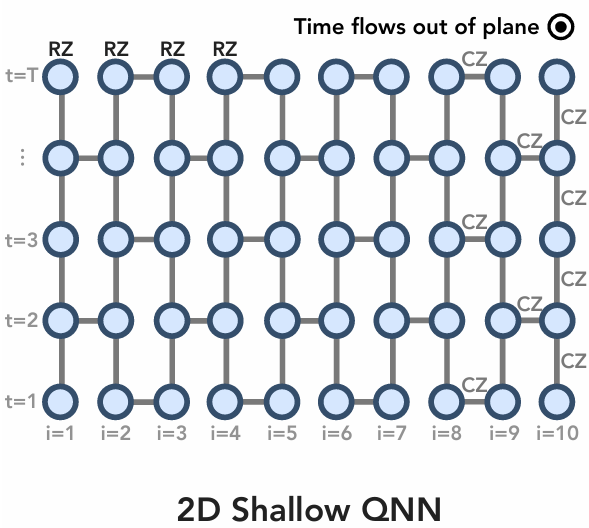
\includegraphics[width=0.98\linewidth,height=0.58\textheight,keepaspectratio]{./assets/2D Shallow QNN.png}

    \vspace{0.35em}
    {\scriptsize 2D shallow QNN architecture used by IDQNN.}

    \column{0.50\textwidth}
    \centering
    \resizebox{0.98\linewidth}{!}{%
    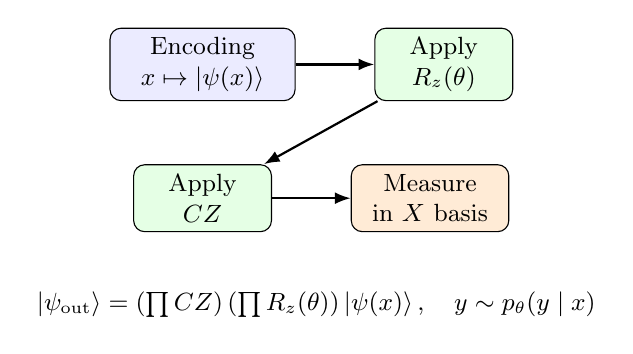
\begin{tikzpicture}[
      font=\small,
      node distance=8mm and 10mm,
      box/.style={draw, rounded corners, minimum width=2.35cm, minimum height=0.85cm, align=center, fill=blue!8},
      op/.style={draw, rounded corners, minimum width=1.75cm, minimum height=0.85cm, align=center, fill=green!10},
      meas/.style={draw, rounded corners, minimum width=2.0cm, minimum height=0.85cm, align=center, fill=orange!16},
      arrow/.style={-{Latex[length=2mm]}, thick}
    ]
      % 2x2 layout
      \node[box] (enc) {Encoding\\$x\mapsto \ket{\psi(x)}$};
      \node[op, right=of enc] (rz) {Apply\\$R_z(\theta)$};
      \node[op, below=of enc] (cz) {Apply\\$CZ$};
      \node[meas, right=of cz] (mx) {Measure\\in $X$ basis};

      % flow: top row -> down -> bottom row
      \draw[arrow] (enc) -- (rz);
      \draw[arrow] (rz) -- (cz);
      \draw[arrow] (cz) -- (mx);

      \node[align=center] at ($(cz)!0.5!(mx)+(0,-1.35)$)
      {$\ket{\psi_{\mathrm{out}}}=\left(\prod CZ\right)\left(\prod R_z(\theta)\right)\ket{\psi(x)},\quad y\sim p_\theta(y\mid x)$};
    \end{tikzpicture}%
    }
  \end{columns}

  \vspace{0.35em}
  \begin{block}{Input-state encoding rule}
    {\footnotesize Qubit $i$ is initialized from
    $\{|0\rangle, |+\rangle=\tfrac{1}{\sqrt{2}}(|0\rangle+|1\rangle)\}$ according to bit $x_i$:
    $0\mapsto|+\rangle,\;1\mapsto|0\rangle$.}
  \end{block}
\end{frame}

\begin{frame}{Task 1 Learning Algorithm: Dataset Construction}
  \begin{enumerate}
    \item Sample $N_{\mathrm{sample}}$ input bitstrings from $D(x)$.
    \item Fix ideal parameters $\theta_{\mathrm{real}}$.
    \item Generate the dataset under ideal parameters:
    \[
      \mathcal D = \{(x_i,y_i)\}_{i=1}^{N_{\mathrm{sample}}}.
    \]
  \end{enumerate}

  \vspace{0.25em}
  \begin{block}{Training objective}
    Estimate $\theta$ from $\mathcal D$ such that $\theta$ approaches $\theta_{\mathrm{real}}$.
  \end{block}
\end{frame}

\begin{frame}{Task 1 Learning Algorithm: Block-wise Estimation}
  \small
  {\bfseries Core idea: estimate each parameter position block-wise.}
  \begin{itemize}
    \item For each parameter at position $(i,j)$, filter samples satisfying:
    \[
      x_{i,j}=0,\qquad x_{\mathcal N(i,j)}=1,
    \]
    where $\mathcal N(i,j)$ denotes positions connected via CZ gates.
    \item Compute the parameter estimate from the filtered samples using the prescribed formula.
  \end{itemize}

  \[
    \hat\theta_{i,j}=\arccos\!\left(1-\frac{2}{N_{\mathrm{sp}}}\sum_{t=1}^{N_{\mathrm{sp}}}y^{(i,j)}_{(t)}\right).
  \]
\end{frame}

\begin{frame}{Proof Sketch  (IDQNN)}
  \small
  \begin{columns}[T,onlytextwidth]
    \column{0.42\textwidth}
    \begin{itemize}
      \item Focus on parameter at position $(i,j)$.
      \item Filtering condition: $x_{i,j}=0$ and neighbors in $\mathcal N(i,j)$ are $1$.
      \item This simplifies the local input to
      \[
        \ket{0}_{i,j-1}\ket{+}_{i,j}\ket{0}_{i,j+1}.
      \]
      \item Measure qubit $(i,j)$ in the $X$ basis.
    \end{itemize}

    \column{0.56\textwidth}
    \vspace{-0.2em}
    \[
      \ket{\psi'}=
      \ket{0}_{i,j-1}
      \left(\ket{+}_{i,j}\cos\frac{\theta_{i,j}}{2}
      -\ket{-}_{i,j}\sin\frac{\theta_{i,j}}{2}\right)
      \ket{0}_{i,j+1}
    \]
    \[
      \Pr\big(y_{i,j}=1\big)=\frac{1-\cos\theta_{i,j}}{2}
    \]
    \begin{alertblock}{Estimator form}
      \[
        \hat\theta_{i,j}=arccos\!\left(1-\frac{2}{N_{\mathrm{sp}}}\sum_{t=1}^{N_{\mathrm{sp}}}y^{(i,j)}_{(t)}\right)
      \]
    \end{alertblock}
  \end{columns}
\end{frame}

\begin{frame}{ Code Result}
  I set $n=12;n_1=3,m=4$; the distance is defined as $d=\max |\cos\hat{\theta}_{i,j}-\cos\theta_{i,j}^{\text{real}}|$.
  \begin{columns}[c,onlytextwidth]
    \column{0.48\textwidth}
    \centering
    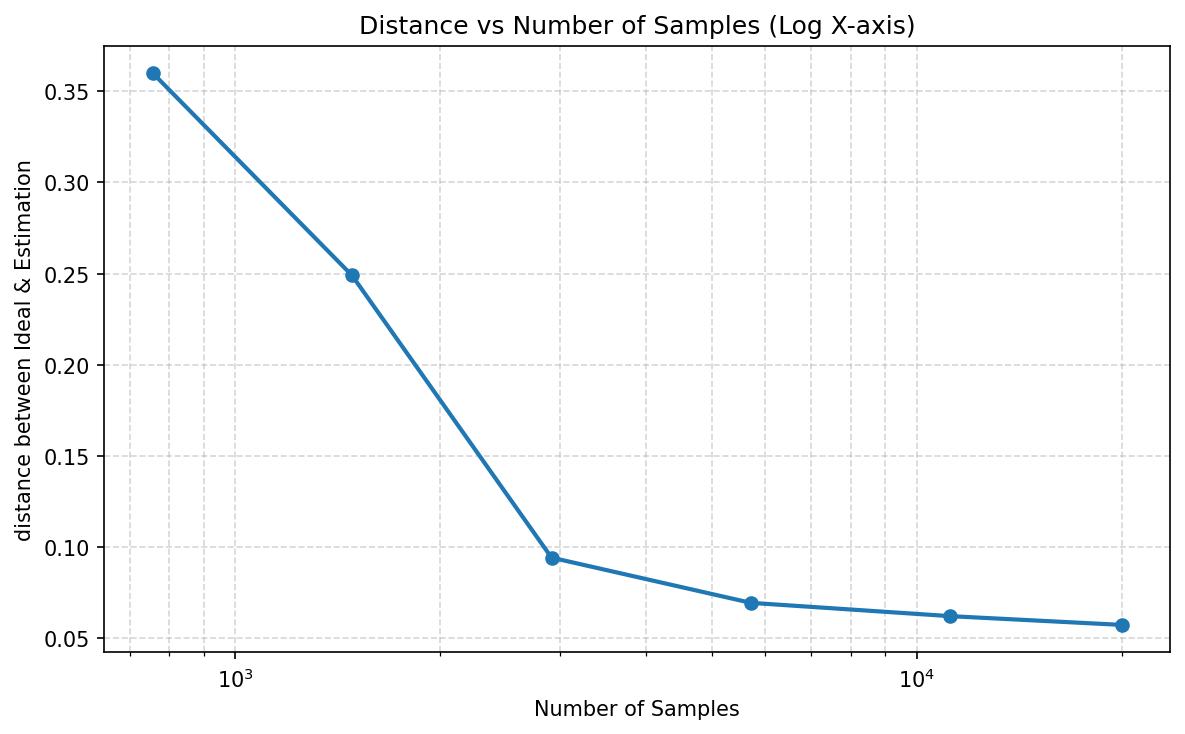
\includegraphics[width=0.98\linewidth,height=0.62\textheight,keepaspectratio]{./assets/distance_vs_samples_logx.png}

    \vspace{0.25em}
    {\scriptsize  Code result: distance vs number of samples (log-scale x-axis).}

    \column{0.48\textwidth}
    \centering
    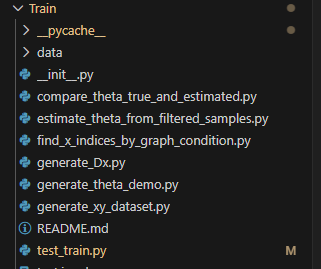
\includegraphics[width=0.98\linewidth,height=0.62\textheight,keepaspectratio]{./assets/python.png}

    \vspace{0.25em}
    {\scriptsize Python implementation screenshot/result.}
  \end{columns}
\end{frame}

\section{Task 1 Experiments \& Results (to be extended)}

\begin{frame}{Hardware Experiment Setting (Authors' Result)}
  \begin{itemize}
    \item The authors implement deep circuit forms on a superconducting quantum processor:
    \begin{itemize}
      \item 68 physical qubits,
      \item 12 rounds (layers) of execution.
    \end{itemize}
    \item This corresponds to a shallow equivalent structure on 816 qubits ($68\times 12$).
  \end{itemize}

  \begin{block}{Implementation trick}
    They bypass mid-circuit measurement by evaluating hardware only for $x=000\cdots0$ and randomly initializing all but the final layer of $y$.
  \end{block}
\end{frame}

\begin{frame}{Device Mapping and Errors}
  \begin{columns}[c,onlytextwidth]
    \column{0.48\textwidth}
    \centering
    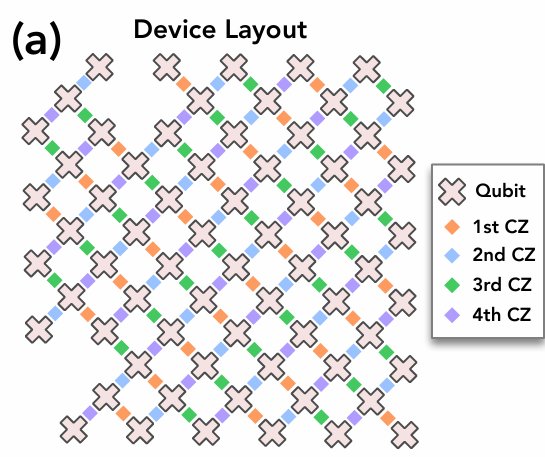
\includegraphics[width=0.98\linewidth,height=0.62\textheight,keepaspectratio]{./assets/2.a.png}
    
    \vspace{0.25em}
    {\scriptsize (a) Around-CZ-gates device layout: 68 physical qubits, mapped to up to 816 shallow qubits.}

    \column{0.48\textwidth}
    \centering
    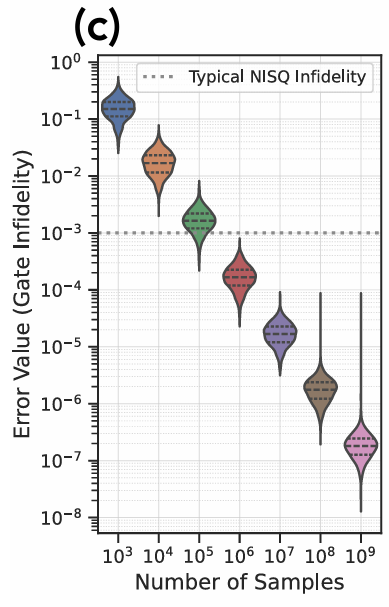
\includegraphics[width=0.98\linewidth,height=0.62\textheight,keepaspectratio]{./assets/2.c.png}

    % \vspace{0.25em}
    % {\scriptsize (c) Classical sample complexity vs gate fidelity.}
  \end{columns}

 
\end{frame}

\begin{frame}{ XEB Performance on Hardware}
  \begin{columns}[c,onlytextwidth]
    \column{0.58\textwidth}
    \centering
    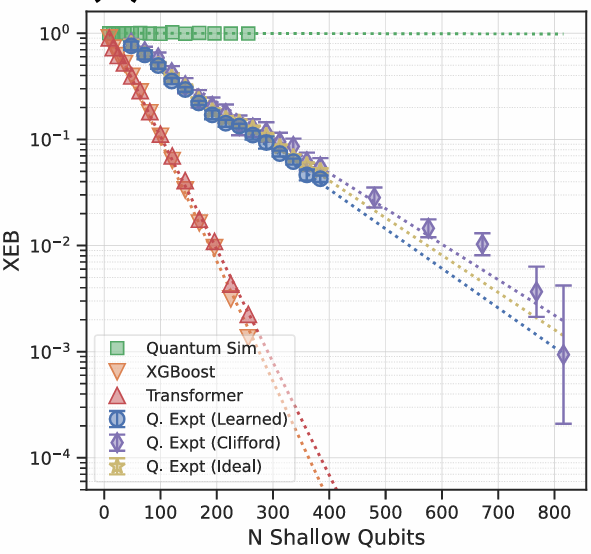
\includegraphics[width=0.98\linewidth,height=0.72\textheight,keepaspectratio]{./assets/2.d.png}

    \column{0.38\textwidth}
    \small
    $$\operatorname*{XEB}=2^n\frac{1}{N}\sum_{i=1}^N P_{ideal}(y_i)-1$$
    \begin{itemize}
      \item Quantum and classical models are compared using Cross-Entropy Benchmarking score.
      \item Inference is evaluated at input bitstring $x=000\cdots0$.
      \item The same datasets are supplied to classical models (Transformer and XGBoost)  
    \end{itemize}
  \end{columns}
\end{frame}

\begin{frame}{ Beyond-Classical Regime}
  \begin{columns}[c,onlytextwidth]
    \column{0.62\textwidth}
    \centering
    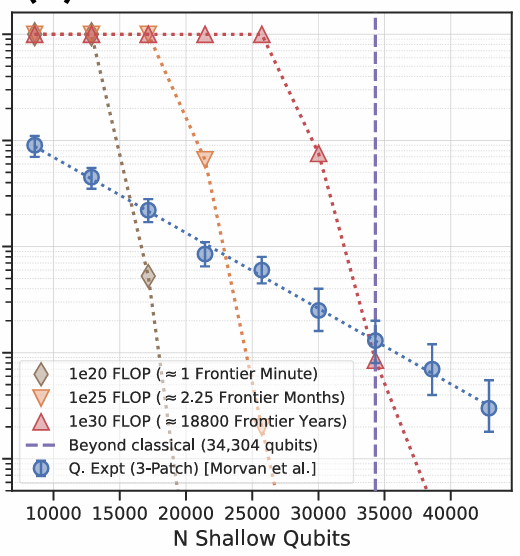
\includegraphics[width=0.98\linewidth,height=0.72\textheight,keepaspectratio]{./assets/2.e.png}

    \column{0.34\textwidth}
    \small
    \begin{itemize}
      \item Performance is inferred in the beyond-classical regime.
    \end{itemize}
  \end{columns}
\end{frame}


\section{Task 2: Learn Quantum Circuits for Accelerated Physical Simulation}

% \begin{frame}{Task 2 (Placeholder)}
%   \begin{block}{Goal}
%     Learn quantum circuits for accelerated physical simulation.
%   \end{block}

%   \begin{itemize}
%     \item Uses a learning algorithm different from Task 1.
%     \item Placeholder for task definition, loss function, hardware setup, and results.
%   \end{itemize}
% \end{frame}


\end{document}
